%%
%% This is file `sample-sigconf.tex',
%% generated with the docstrip utility.
%%
%% The original source files were:
%%
%% samples.dtx  (with options: `sigconf')
%% 
%% IMPORTANT NOTICE:
%% 
%% For the copyright see the source file.
%% 
%% Any modified versions of this file must be renamed
%% with new filenames distinct from sample-sigconf.tex.
%% 
%% For distribution of the original source see the terms
%% for copying and modification in the file samples.dtx.
%% 
%% This generated file may be distributed as long as the
%% original source files, as listed above, are part of the
%% same distribution. (The sources need not necessarily be
%% in the same archive or directory.)
%%
%% The first command in your LaTeX source must be the \documentclass command.

\newcommand{\NPM}{NPM}
\newcommand{\NodeJS}{NodeJS}

% Result numbers: Check `numbers.log` in `dts-generate-results' repo
\newcommand{\CountTotalModulesDefinitelyTyped}{6029}
\newcommand{\CountModulesWithRepositoryUrl}{4974}
\newcommand{\CountModulesWithReadmeFile}{4292}
\newcommand{\CountModulesWithCodeExamples}{2260}
\newcommand{\CountModulesWorkingCodeExamples}{946}
\newcommand{\CountModulesRunTimeInfoExtracted}{436}
\newcommand{\CountModulesGeneratedDeclarationFile}{249}
\newcommand{\CountModulesOnlySolvableDifferences}{111}

% Result helper numbers
\newcommand{\CountModulesWithoutReadmeFile}{682} % \CountModulesWithRepositoryUrl{} - \CountModulesWithReadmeFile{}
\newcommand{\CountModulesNotWorkingCodeExamples}{1314} % \CountModulesWithCodeExamples{} - \CountModulesWorkingCodeExamples{}
\newcommand{\CountModulesRunTimeInfoCouldNotBeExtracted}{510} % \CountModulesWorkingCodeExamples{} - \CountModulesRunTimeInfoExtracted{}
\newcommand{\CountModulesDeclarationFileCouldNotBeGenerated}{138} % \CountModulesGeneratedDeclarationFile{} - \CountModulesOnlySolvableDifferences{}
\newcommand{\secref}[1]{Section~\ref{#1} - \nameref{#1}}
\newcommand{\figref}[1]{Figure~\ref{#1}}
\newcommand{\coderef}[1]{Listing~\ref{#1}}


\documentclass[sigconf]{acmart}
\usepackage{listings}

\usepackage{cleveref}
\usepackage{pgfplots}
\usepackage{tikz}
\usetikzlibrary{positioning}

\usepackage{xcolor}
\usepackage{tcolorbox}
\tcbuselibrary{breakable}

\usepackage{subcaption}

\usepackage[htt]{hyphenat}

\definecolor{backgroundgray}{rgb}{.94,.94,.94}

\lstdefinelanguage{JavaScript}{
  keywords={typeof, new, true, false, catch, function, return, null, catch, switch, var, if, in, while, do, else, case, break, undefined,const},
  keywordstyle=\color{black}\bfseries,
  ndkeywords={class, export, boolean, throw, implements, import, this},
  ndkeywordstyle=\color{black}\bfseries,
  identifierstyle=\color{darkgray},
  sensitive=false,
  comment=[l]{//},
  morecomment=[s]{/*}{*/},
  commentstyle=\color{lightgray}\slshape,
  stringstyle=\color{darkgray}\ttfamily,
  morestring=[b]',
  morestring=[b]"
}

\lstdefinelanguage{TypeScript}{
  keywords={typeof, new, true, false, catch, function, return, null, catch, switch, var, if, in, while, do, else, case, break, undefined,const},
  keywordstyle=\color{black}\bfseries,
  ndkeywords={class, export, boolean, throw, implements, import, this, declare, constructor, namespace, interface},
  ndkeywordstyle=\color{black}\bfseries,
  identifierstyle=\color{darkgray},
  sensitive=false,
  comment=[l]{//},
  morecomment=[s]{/*}{*/},
  commentstyle=\color{lightgray}\slshape,
  stringstyle=\color{darkgray}\ttfamily,
  morestring=[b]',
  morestring=[b]"
}

\lstset{
   backgroundcolor=\color{backgroundgray},
   extendedchars=true,
   basicstyle=\footnotesize\ttfamily,
   showstringspaces=false,
   showspaces=false,
   numbers=none,
   numberstyle=\footnotesize,
   numbersep=9pt,
   tabsize=2,
   breaklines=true,
   showtabs=false
}

\graphicspath{{./graphics/}}%helpful if your graphic files are in another directory

\settopmatter{printfolios=true}
%%
%% \BibTeX command to typeset BibTeX logo in the docs
\AtBeginDocument{%
  \providecommand\BibTeX{{%
    \normalfont B\kern-0.5em{\scshape i\kern-0.25em b}\kern-0.8em\TeX}}}

%% Rights management information.  This information is sent to you
%% when you complete the rights form.  These commands have SAMPLE
%% values in them; it is your responsibility as an author to replace
%% the commands and values with those provided to you when you
%% complete the rights form.

% \setcopyright{acmcopyright}
% \copyrightyear{2018}
% \acmYear{2018}
% \acmDOI{10.1145/1122445.1122456}

%% These commands are for a PROCEEDINGS abstract or paper.
% \acmConference[Woodstock '18]{Woodstock '18: ACM Symposium on Neural
%   Gaze Detection}{June 03--05, 2018}{Woodstock, NY}
% \acmBooktitle{Woodstock '18: ACM Symposium on Neural Gaze Detection,
%   June 03--05, 2018, Woodstock, NY}
% \acmPrice{15.00}
% \acmISBN{978-1-4503-XXXX-X/18/06}

%%
%% Submission ID.
%% Use this when submitting an article to a sponsored event. You'll
%% receive a unique submission ID from the organizers
%% of the event, and this ID should be used as the parameter to this command.
%%\acmSubmissionID{123-A56-BU3}

%%
%% The majority of ACM publications use numbered citations and
%% references.  The command \citestyle{authoryear} switches to the
%% "author year" style.
%%
%% If you are preparing content for an event
%% sponsored by ACM SIGGRAPH, you must use the "author year" style of
%% citations and references.
%% Uncommenting
%% the next command will enable that style.
%%\citestyle{acmauthoryear}

%%
%% end of the preamble, start of the body of the document source.
\begin{document}

%%
%% The "title" command has an optional parameter,
%% allowing the author to define a "short title" to be used in page headers.
\title{Generation of TypeScript Declaration Files from JavaScript Code}

%%
%% The "author" command and its associated commands are used to define
%% the authors and their affiliations.
%% Of note is the shared affiliation of the first two authors, and the
%% "authornote" and "authornotemark" commands
%% used to denote shared contribution to the research.

\author{Fernando Cristiani}
\affiliation{%
  \institution{Hochschule Karlsruhe}
  \city{Karlsruhe}
  \country{Germany}}
\email{fernando.cristiani@hs-karlsruhe.de}

\author{Peter Thiemann}
\affiliation{%
  \institution{Albert-Ludwigs-Universit{\"a}t Freiburg}
  \city{Freiburg}
  \country{Germany}
}
\email{thiemann@informatik.uni-freiburg.de}


%%
%% By default, the full list of authors will be used in the page
%% headers. Often, this list is too long, and will overlap
%% other information printed in the page headers. This command allows
%% the author to define a more concise list
%% of authors' names for this purpose.
% \renewcommand{\shortauthors}{Trovato and Tobin, et al.}

%%
%% The abstract is a short summary of the work to be presented in the
%% article.
\begin{abstract}
  Developers are starting to write large and complex applications in
  TypeScript, a typed dialect of JavaScript. TypeScript applications
  integrate JavaScript libraries via typed descriptions of their APIs
  called declaration files. DefinitelyTyped is the standard public
  repository for these files.
  The repository is populated and maintained manually by volunteers, which
  is error prone and time consuming. Discrepancies between a
  declaration file and the JavaScript implementation lead to
  incorrect feedback from the TypeScript IDE and thus to incorrect uses
  of the underlying JavaScript library.

  This work presents \texttt{dts-generate}, a tool that generates
  TypeScript declaration files for JavaScript libraries uploaded to the \NPM{}
  registry. It extracts code examples from the documentation written by
  the developer, executes the library driven by the examples, gathers
  run-time information, and generates a declaration file based on this
  information. To evaluate the tool, \CountModulesGeneratedDeclarationFile{} declaration files were
  generated directly from an \NPM{} module and \CountModulesOnlySolvableDifferences{} of these were
  compared with the corresponding declaration file provided on
  DefinitelyTyped.  All these files either
  exhibited no differences at all or differences that can be resolved by
  extending the developer-provided examples.
\end{abstract}

%%
%% The code below is generated by the tool at http://dl.acm.org/ccs.cfm.
%% Please copy and paste the code instead of the example below.
%%
% \begin{CCSXML}
% <ccs2012>
%  <concept>
%   <concept_id>10010520.10010553.10010562</concept_id>
%   <concept_desc>Computer systems organization~Embedded systems</concept_desc>
%   <concept_significance>500</concept_significance>
%  </concept>
%  <concept>
%   <concept_id>10010520.10010575.10010755</concept_id>
%   <concept_desc>Computer systems organization~Redundancy</concept_desc>
%   <concept_significance>300</concept_significance>
%  </concept>
%  <concept>
%   <concept_id>10010520.10010553.10010554</concept_id>
%   <concept_desc>Computer systems organization~Robotics</concept_desc>
%   <concept_significance>100</concept_significance>
%  </concept>
%  <concept>
%   <concept_id>10003033.10003083.10003095</concept_id>
%   <concept_desc>Networks~Network reliability</concept_desc>
%   <concept_significance>100</concept_significance>
%  </concept>
% </ccs2012>
% \end{CCSXML}

% \ccsdesc[500]{Computer systems organization~Embedded systems}
% \ccsdesc[300]{Computer systems organization~Redundancy}
% \ccsdesc{Computer systems organization~Robotics}
% \ccsdesc[100]{Networks~Network reliability}

%%
%% Keywords. The author(s) should pick words that accurately describe
%% the work being presented. Separate the keywords with commas.
\keywords{JavaScript, TypeScript, Dynamic Analysis, Declaration Files}

%% A "teaser" image appears between the author and affiliation
%% information and the body of the document, and typically spans the
%% page.
% \begin{teaserfigure}
%   GRAPHICS REMOVED % \includegraphics[width=\textwidth]{sampleteaser}
%   \caption{Seattle Mariners at Spring Training, 2010.}
%   \Description{Enjoying the baseball game from the third-base
%   seats. Ichiro Suzuki preparing to bat.}
%   \label{fig:teaser}
% \end{teaserfigure}

%%
%% This command processes the author and affiliation and title
%% information and builds the first part of the formatted document.
\maketitle

\section{Introduction}
\label{sec:introduction}
JavaScript is the most popular language for writing web
applications \cite{github-statistics}. It is also increasingly used
for back-end applications running in \NodeJS{}, a JavaScript-based
server-side platform. JavaScript is appealing to developers because
its forgiving dynamic typing enables 
them to create simple pieces of code very quickly and proceed on a
trial-and-error basis.

JavaScript was never intended to be more than a
scripting language and thus lacks features for maintaining and evolving large
codebases. However, nowadays developers create large and complex
applications in JavaScript. 
Mistakes such as mistyped property
names and misunderstood or unexpected type coercions cause developers
to spend a significant amount of time in debugging. There is ample
evidence for such mishaps. For example, a 
JavaScript code blog\footnote{\url{https://wtfjs.com}} collects experiences
from developers facing unexpected situations while programming in
JavaScript. \coderef{code:introduction-javascript-wtfs} exposes some
of these unintuitive JavaScript behaviors. 

\begin{lstlisting}[
  caption={\textbf{Unintuitive JavaScript behavior:} Falsy values,
  \lstinline!null! vs. \lstinline!undefined!,
\lstinline!typeof!, and type coercion},
  language=JavaScript,
label=code:introduction-javascript-wtfs,
  float=bp,
  captionpos=b
]
"0" == false; // true
true == "1.00"; // true
false == "    \n\r\t     "; // true
false == []; // true
0 == []; // true
null == undefined; // true
null + undefined + [1, 2, 3] // 'NaN1,2,3' 
typeof null; // object
null instanceof Object; // false
[1] + 1; //'11'
[2] == "2"; // true
"hello world".lenth + 1 // NaN | note 'lenth' instead of 'length'
[1, 15, 20, 100].sort() // [ 1, 100, 15, 20 ]
\end{lstlisting}

The cognitive load produced by these behaviors is mitigated in languages that use
build tools based on type information. This insight motivated the
creation of TypeScript, a superset of JavaScript with expressive type
annotations \cite{typescript}. It has become a widely used alternative
among JavaScript developers, because it incorporates features that are
helpful for developing and maintaining large applications
\cite{DBLP:conf/icse/GaoBB17}. TypeScript enables the early detection
of several kinds of run-time errors and the integration of code intelligence
tools like autocompletion in an IDE.

Despite the advantages, it is unrealistic to expect the world to
switch to TypeScript in a day. Therefore, 
existing JavaScript libraries can be used in a TypeScript project by
adding a declaration file that contains a description of the library's
API in terms of types. 
The DefinitelyTyped repository~\cite{definitely-typed-repository} has
been created as a community effort to collect declaration files for
popular JavaScript libraries. At the time of writing it contains
declaration files for more than 6000 libraries.

Unfortunately, creation and maintenance of most declaration
files in DefinitelyTyped is conducted manually,
which is time consuming and  error prone. Errors are aggravated because TypeScript takes a
declaration file at face value. Discrepancies between declaration and
implementing JavaScript library are not detected at 
compile time and result in incorrect behavior (e.g., autocompletion
hints) of the IDE. 
As TypeScript does not perform any run-time 
checking of types, these  discrepancies can lead to unexpected 
behavior and crashes. This kind of experience can lead to longish debugging sessions,  developer
frustration, and decreasing confidence in the tool chain.

\subsection{Approach}
\label{sec:approach}

% I think the reader gets the impression from the text that obtaining the code examples
% is a "main feature" of our tool, where in fact it is only a way of easily obtaining
% runtime information to execute our tool. We could've followed the approach of obtaining
% the runtime information from the tests.
% This can be useful also to divert the attention from how many repositories had README files, etc.
% After using the code examples, we also found out that they provided a useful approximation
% not only on the input types but also on how to use the library (i.e. we don't analyze the structure of the library).
% This is a useful insight which can be used later to infer the correct types.
%
% Should we change this to 'we rely on runtime information'. 'We used the examples
% provided by the developer as part of the documentation of a library as a first
% pragmatic way of obtaining runtime information'.
We aim to improve on this situation by providing a tool that generates
TypeScript declaration files automatically. To do so, we rely on the examples provided
by the developer as part of the documentation of a library. If these
examples are sufficiently rich, then our toolchain can generate
high-quality declaration files for the library. This way we take
advantage of 
best practices in the dynamic languages community which favors
examples and tests over writing out type signatures.

As an example, consider the NPM\footnote{NPM is the \href{https://www.npmjs.com/}{Node package
  manager}, an online repository for JavaScript modules.} module
\texttt{abs} that
``computes the absolute path of an input''. Its documentation contains
the following three
examples\footnote{\url{https://www.npmjs.com/package/abs}}. 

\begin{lstlisting}[language=JavaScript,numbers=none]
const abs = require("abs");
 
console.log(abs("/foo"));
// => "/foo"
 
console.log(abs("foo"));
// => "/path/to/where/you/are/foo"
 
console.log(abs("~/foo"));
// => "/home/username/foo"
\end{lstlisting}
From the examples, our tool generates the following TypeScript declaration file.
\begin{lstlisting}[language=TypeScript,numbers=none]
export = Abs;
declare function Abs(input: string): string;
\end{lstlisting}
It used to be equivalent to the declaration file provided in the
DefinitelyTyped
repository\footnote{\url{https://github.com/DefinitelyTyped/DefinitelyTyped/blob/master/types/abs/index.d.ts}},
but the maintainer indicates (since May 10, 2021) that the parameter is optional:
\begin{lstlisting}[language=TypeScript,numbers=none]
declare function abs(input?: string): string;
export = abs;
\end{lstlisting}
This case is quite frequent. The information in our declaration file is
correct, but incomplete, because the developers did not document the
fact that the input is optional. If the developer had provided the
call  \lstinline/abs()/ as an additional 
example, then our tool would have generated exactly
the declaration on DefinitelyTyped! We call this case a solvable
difference between our tool's output and the DefinitelyTyped
declaration file.

% \begin{description}
% \item[PJT: maybe later] Some previous work tackled the problem of improving
%   the quality of declaration files. Feldthaus et al
%   \cite{DBLP:conf/oopsla/FeldthausM14} search automatically for
%   mismatches between a declaration file and implementation
%   code. TSTest \cite{DBLP:journals/pacmpl/KristensenM17} adapted
%   feedback-directed random testing to detect discrepancies between a
%   declaration file and a JavaScript library. Tools like TSInfer and
%   TSEvolve~\cite{DBLP:conf/fase/KristensenM17} are designed for
%   assisting the creation of new declaration files and supporting the
%   evolution the declaration file when the corresponding JavaScript
%   library gets modified, respectively. They rely on an existing static
%   analyzer for JavaScript \cite{DBLP:conf/sas/JensenMT09}.  TypeScript
%   itself developed \texttt{dts-gen}, a tool that generates a
%   declaration file that is meant to be used as a \emph{starting point
%     for writing a high-quality declaration file} \cite{dts-gen}.
% \end{description}

Our tool \texttt{dts-generate} is a first step to explore the possibilities for
generating useful declaration files from code
examples.
% Should we change it to 'explore the possibilities for
% generating useful declaration files from runtime information'.

\texttt{dts-generate} comes with a framework that 
supports the generation of declaration files for an existing
JavaScript library published to the \NPM{} registry. The tool gathers
data flow and type information at run time to generate a declaration
file based on that information.

The novelty of our tool is twofold:
\begin{enumerate}
\item
  %% without the heavy lifting of static analysis
  We do not rely on static analysis, which is hard to implement
  soundly and precisely and which is prone to maintenance problems
  when keeping up with JavaScript's frequent language updates.
\item
  We extract example code from the programmer's library
  documentation and rely on dynamic analysis to extract typed usage
  patterns for the library from the example runs.
\end{enumerate}
% The architecture supports the future incorporation of a Symbolic
% Execution Engine that expands the initial code base using the
% signatures in the declaration file. The iterative process of exploring
% new execution paths will refine the generated declaration file in each
% iteration. 

% Finally, we generated declaration files for \CountModulesGeneratedDeclarationFile{} JavaScript libraries
% and evaluated them against the DefinitelyTyped repository. 

The implementation and the results are available in the following repositories:

\begin{itemize}
  \item \url{https://github.com/proglang/run-time-information-gathering/tree/v1.1.0}
  \item \url{https://github.com/proglang/ts-declaration-file-generator/tree/v1.5.0}
  \item \url{https://github.com/proglang/ts-declaration-file-generator-service/tree/v1.2}
  \item \url{https://github.com/proglang/dts-generate-method/tree/v1.3.1}
  \item \url{https://github.com/proglang/dts-generate-results/tree/v1.4.0}
\end{itemize}

\subsection{Contributions}
\label{sec:contributions}


\begin{itemize}
% \item We introduce an architecture that supports generating TypeScript
%   Declaration Files for a given JavaScript Library using run-time
%   information. The architecture supports the future incorporation of a
%   Symbolic Execution Engine that expands the initial code base using
%   the signatures in the declaration file. The iterative process of
%   exploring new execution paths will refine the generated declaration
%   file in each iteration.
\item A framework that extracts code examples from the
  documentation of an \NPM{} package and collects run-time type
  information from running these examples (Sections~\ref{sec:initial-code-base}
  and~\ref{sec:run-time-information}). 

\item Design and implementation of the tool \texttt{dts-generate}, a command line
  application that generates a valid TypeScript declaration file for
  an \NPM{} package using run-time information
  (Section~\ref{sec:typescr-decl-file}). 

\item A comparator for TypeScript declaration files
  (Section~\ref{sec:dts-compare}) for evaluating our framework and to
  detect   incompatibilities when evolving JavaScript modules.
\item An evaluation of our framework (Sections~\ref{sec:dts-generate-evaluation}
  and~\ref{sec:results}). We examined all \CountTotalModulesDefinitelyTyped{} entries in 
  the DefinitelyTyped repository and found \CountModulesGeneratedDeclarationFile{} sufficiently
  well documented \NPM{} packages, on which we ran \texttt{dts-generate}
  and compared the outcome with the respective declaration file from the
  DefinitelyTyped repository. 
\end{itemize}

\section{Motivating Example}
\label{sec:motivating-example}
The \NPM{} package \texttt{glob-to-regexp} provides functionality to turn a
glob expression for matching filenames in the shell into a regular
expression\footnote{\url{https://www.npmjs.com/package/glob-to-regexp}}. It 
has about 9.9M weekly downloads and 188 \NPM{} packages depend on it. If
a developer creates or extends TypeScript code that depends on the
\texttt{glob-to-regexp} library, the TypeScript
compiler and IDE require a declaration file for that library to
perform static checking and code completion, respectively. With
\texttt{dts-generate} we automatically generate a TypeScript
declaration file for \texttt{glob-to-regexp}. Our tool downloads the \NPM{} 
package, runs the examples extracted from its documentation, gathers
run-time information, and generates a TypeScript declaration
file. The result is 
shown in \figref{fig:motivating-example-glob-to-regexp-vscode} and it is
ready for use in a TypeScript project. For example,  Visual Studio's
code completion runs properly with the generated file
(\figref{fig:motivating-example-glob-to-regexp-vscode}). If the
\texttt{glob-to-regexp} package gets modified in the future, a new declaration
file can be generated automatically using
\texttt{dts-generate}. Our comparator tool (Section~\ref{sec:dts-compare}) can compare the new file
for incompatibilities with the previous declaration file.

\begin{figure}[tp]
  \centering
%  \begin{subfigure}{0.70\linewidth}
    \begin{lstlisting}[language=TypeScript,numbers=none]
export = GlobToRegexp;

declare function GlobToRegexp(
    glob: string, 
    opts?: GlobToRegexp.I__opts): RegExp;
declare namespace GlobToRegexp {
  export interface I__opts {
    'extended'?: boolean;
    'globstar'?: boolean;
    'flags'?: string;
  }

}
    \end{lstlisting}
  % \end{subfigure}
  \begin{center}
    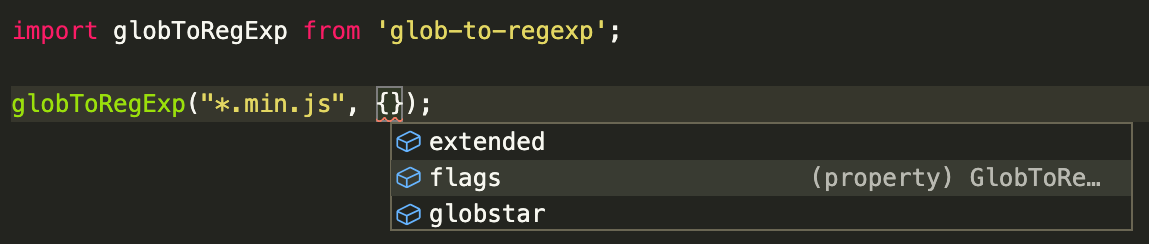
\includegraphics[width=\linewidth]{motivating-example-glob-to-regexp-vscode.png}
  \end{center}

  \caption{Declaration file for \texttt{glob-to-regexp} 
    generated with \texttt{dts-generate} - The interface is
    detected correctly. Optional parameters are detected. The declaration 
    file is usable in Visual Studio Code\protect\footnote{\url{https://code.visualstudio.com}}} 
  \label{fig:motivating-example-glob-to-regexp-vscode}
\end{figure}

% After filling in some background information on declaration files,
% Section~\ref{sec:gener-typescr-decl} examines each step in the
% generation process in detail and refer back to this example for
% concreteness.

\section{TypeScript Declaration Files}
\label{sec:typescr-decl-files}

The declaration file shown in \figref{fig:motivating-example-glob-to-regexp-vscode}
describes a package with a single exported function. The first parameter is of type
\texttt{string} and the second one is an optional object described by an interface. TypeScript namespaces
organize types declared in a declaration file and avoid name clashes with other types
\cite{typescript-namespaces}. For example, the interface
\lstinline[language=TypeScript]{I__opts} is declared in namespace
\lstinline[language=TypeScript]{globToRegexp} in
\figref{fig:motivating-example-glob-to-regexp-vscode}. Hence its uses
must be qualified by the namespace as in
\lstinline[language=TypeScript]{globToRegexp.I__opts}.

This file is an instance of one of the standard templates for writing
declaration
files\footnote{\url{https://www.typescriptlang.org/docs/handbook/declaration-files/templates.html}}:
\textbf{module}, \textbf{module-class}, and
\textbf{module-function}. 
Each template corresponds to a different way of organizing the exports
of a JavaScript library. The choice of the template depends on the
structure of the underlying JavaScript library:
\begin{description}
\item[module] several exported functions,
\item[module-class] a class-like structure,
\item[module-function] exactly one exported function.
\end{description}
There are further templates, but most libraries fall in one of these
three categories.
Both libraries \texttt{glob-to-regexp} and \texttt{abs} are instances of the
\textbf{module-function} template.

\begin{lstlisting}[
  caption={Example for \textbf{module-function} template},
  language=bash,
label=code:dts-generate-example,
  float,captionpos=b
]
$ ./dts-generate abs
$ cat output/abs/index.d.ts 
export = Abs;

declare function Abs(input: string): string;
\end{lstlisting}

\begin{figure*}[t]
\centering
\begin{subfigure}[t]{0.48\linewidth}
  \begin{lstlisting}[language=JavaScript,numbers=none]
var greet = require("./greet-settings-module");

greet({
greeting: "hello world",
duration: 4000
});

greet({
greeting: "hello world",
color: "#00ff00"
});
  \end{lstlisting}
  \caption{Example for \textbf{module-function} template}
  \label{fig:example-module-function}
\end{subfigure}
\hfill
\begin{subfigure}[t]{0.48\linewidth}
  \begin{lstlisting}[language=TypeScript,numbers=none]
export = GreetSettingsModule;

declare function GreetSettingsModule(settings: GreetSettingsModule.I__settings): void;
declare namespace GreetSettingsModule {
export interface I__settings {
  'greeting': string;
  'duration'?: number;
  'color'?: string;
}

}
  \end{lstlisting}
  \caption{Declaration file for \textbf{module-function} template}
  \label{fig:template-module-function}
\end{subfigure}

\begin{subfigure}[t]{0.48\linewidth}
    \begin{lstlisting}[language=JavaScript,numbers=none]
var myLib = require("./greet-module");

var result = myLib.makeGreeting("hello, world");
console.log("The computed greeting is: " + result);

var goodbye = myLib.makeGoodBye();
console.log("The computed goodbye is: " + goodbye);    
    \end{lstlisting}
  \caption{Example for \textbf{module} template}
  \label{fig:example-module}
  \end{subfigure}
  \hfill
  \begin{subfigure}[t]{0.48\linewidth}
    \begin{lstlisting}[language=TypeScript,numbers=none]
export function makeGreeting(str: string): string;
export function makeGoodBye(): string;        
    \end{lstlisting}
    \caption{Declaration file for \textbf{module} template}
    \label{fig:template-module}
  \end{subfigure}

  \begin{subfigure}[t]{0.48\linewidth}
    \begin{lstlisting}[language=JavaScript,numbers=none]
var Greeter = require("./greet-classes-module.js");

var myGreeter = new Greeter("hello, world");
myGreeter.greeting = "howdy";
myGreeter.showGreeting();
    \end{lstlisting}
    \caption{Example for \textbf{module-class} template}
    \label{fig:example-class}
  \end{subfigure}
  \hfill
  \begin{subfigure}[t]{0.48\linewidth}
    \begin{lstlisting}[language=TypeScript,numbers=none]
export = Greeter;

declare class Greeter {
constructor(message: string);
showGreeting(): void;
}

declare namespace Greeter {
}
    \end{lstlisting}
    \caption{Declaration file for \textbf{module-class} template}
    \label{fig:template-class}
  \end{subfigure}

\caption{Example uses and declaration files for different templates}
\label{fig:typescript-templates-by-example}
\end{figure*}

The TypeScript project provides a guide on how to write high-quality declaration
files\footnote{https://www.typescriptlang.org/docs/handbook/declaration-files/by-example.html}. The guide
explains the main concepts through examples. We selected one example for each template
from the guide and
used \texttt{dts-generate} to generate a corresponding declaration file, as shown in
\figref{fig:typescript-templates-by-example}.

Unlike \texttt{dts-gen}, a TypeScript package that generates a template for a declaration
file which only analyzes the structure of the module, we determine the kind of declaration file by examining the usage
of the module. If the
imported entity is used solely as a function as in Figure~\ref{fig:example-module-function}, the
generated declaration file follows the \textbf{module-function} template as shown in Figure~\ref{fig:template-module-function}.
If the example only accesses properties of the imported entity as in
Figure~\ref{fig:example-module}, we generate according to the \textbf{module} template (Figure~\ref{fig:template-module}).
If the imported entity is used with \lstinline/new/ to create new instances as in
Figure~\ref{fig:example-class}, we generate a \textbf{module-class} template (Figure~\ref{fig:template-class}).
While it is possible to create a library of undetermined category, our selection is driven
by the examples in the documentation and 
hence reflects the developers intent.
% Run-time analysis proves useful in this case,
% since it is not sufficient to statically analyze the exported module. 


% \begin{figure}[tp]
%   \centering
%   \begin{subfigure}{0.80\linewidth}
%       \begin{lstlisting}[language=JavaScript]
% var multiPurposeModule = require('./multi-purpose-module');

% // module-function
% console.log(multiPurposeModule("John", "Doe"));
% // John Doe


% // module-class
% var m = new multiPurposeModule("Jane", "Doe");
% console.log(m.firstName + " - " + m.lastName);
% // Jane - Doe

% console.log(m.sayHello());
% // Hello, my name is Jane Doe

% // module
% console.log(multiPurposeModule.anotherFunction());
% // I am another function! 
%       \end{lstlisting}
%       \caption{index.js}
%     \end{subfigure}

%     \begin{subfigure}{0.80\linewidth}
%       \begin{lstlisting}[language=TypeScript,numbers=none]
% var multiPurposeModule = function(firstName, lastName) {
%   this.firstName = firstName;
%   this.lastName = lastName;

%   return firstName + " " + lastName;
% };

% multiPurposeModule.prototype.sayHello = function() {
%   return "Hello, my name is " + this.firstName + " " + this.lastName;
% };

% multiPurposeModule.anotherFunction = function() {
%   return "I am another function!";
% };

% module.exports = multiPurposeModule;   
%       \end{lstlisting}
%       \caption{multi-purpose-module/index.js}
%     \end{subfigure}
%   \caption{Example module that implements all three templates simultaneously}
%   \label{fig:multi-purpose-module-example}
% \end{figure}

\section{The Generation of TypeScript Declaration Files}
\label{sec:gener-typescr-decl}
This section gives an overview of our approach to generating
TypeScript declaration files from a JavaScript library packaged in
\NPM. \figref{fig:tsd_generation_method_block_diagram} gives a rough
picture of the inner working of our tool \texttt{dts-generate}. The
input is an \NPM{} package and the output is a TypeScript declaration
file for the package if it is ``sufficiently documented'', which we
substantiate in the next subsection.

% We introduce \texttt{dts-generate}, a command line tool which
% generates a valid TypeScript Declaration File for a specific
% JavaScript Library uploaded to the \NPM{} Registry, as explained in
% \figref{fig:tsd_generation_method_block_diagram}. The tool is intended
% to be used on existing, published \NPM{} packages. The generated
% output TypeScript declaration file is a valid file which can be used
% for development and uploaded to the DefinitelyTyped Repository. 

\begin{figure}[tp]
  \centering
  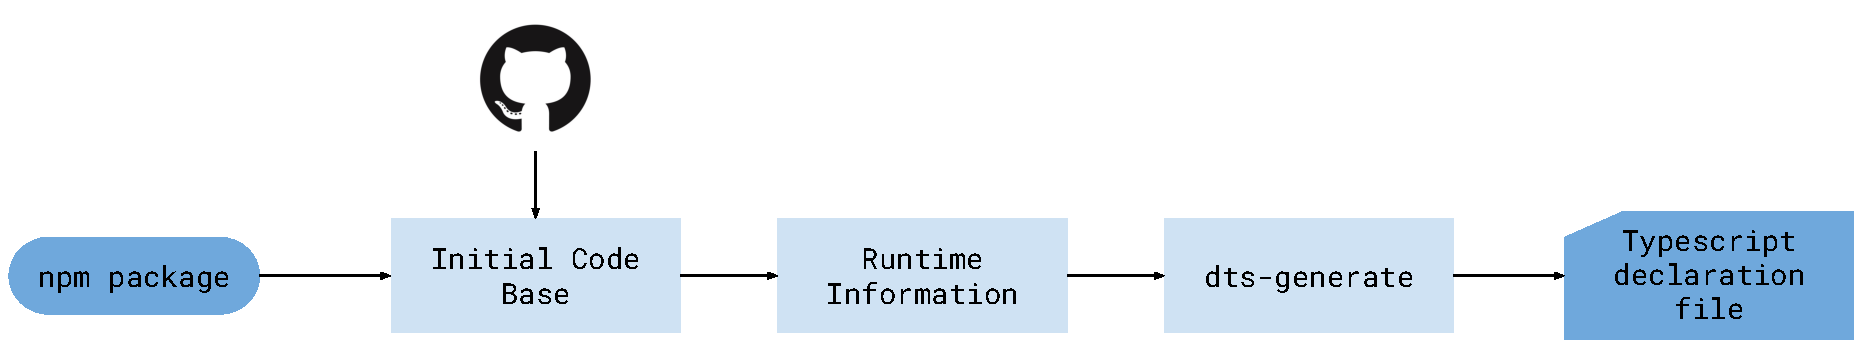
\includegraphics[width=1\linewidth]{dts-generate-block-diagram.pdf}
  \caption[dts-generate - Architecture overview]{dts-generate - Architecture
      overview - The initial code base is retrieved from the \NPM{} package's
    repository.
    Run-time information is gathered driven by example code.
    A TypeScript Declaration File is generated using run-time
    information.
    % A Symbolic Execution Engine creates test cases based on the generated
    % Declaration File and via a feedback loop enriches the code base until the stopping
    % criteria is reached.
    % The final TypeScript Declaration File gets returned.
    % Feedback
    % loop through the Symbolic Execution Engine was not implemented. It can be added in a
    % future to the existing architecture, without modifying the working blocks.
  } 
  \label{fig:tsd_generation_method_block_diagram}
\end{figure}

As \texttt{dts-generate} is based on run-time information, 
exemplary code fragments that execute the JavaScript library are
needed to obtain 
significant run-time information from running the instrumented library
code.


The examples and the code base of the library are instrumented with
Jalangi \cite{DBLP:conf/sigsoft/SenKBG13} to gather data flow
information and type information at run time. Jalangi is a configurable
framework for dynamic analysis of JavaScript. It provides several
analysis modules that we extended as needed to retrieve the required
run-time information.
%, which is then saved in a JSON file. 

A second independent block uses the run-time information to generate a
TypeScript declaration file. It infers the overall structure of the JavaScript
library, its interfaces, and the types from the run-time information. 
The resulting declaration file is ready for use in the development
process. Its contents mimic the usage of the library in the example
code fragments and match the structure of the
JavaScript library under analysis, so that the JavaScript code
generated after compiling the TypeScript code runs without
interface-related errors.

The command-line interface is very simple and inspired by the \texttt{dts-gen} tool
\cite{dts-gen} (see \coderef{code:dts-generate-example}). The only required
argument is the name of the module published to the \NPM{} registry. 

\subsection{Initial Code Base}
\label{sec:initial-code-base}

To extract run-time information from a JavaScript library, it is
necessary, by definition, to execute the code, because the
analysis modules provided by Jalangi can only gather information if the instrumented code gets executed.

There are several options to obtain code fragments that drive the
library code:
\begin{enumerate}
\item\label{item:1} execute code that imports the library;
\item\label{item:2} execute the test cases that come with the library;
\item\label{item:3} execute code fragments extracted from the library documentation.
\end{enumerate}

Option~\ref{item:1} does not solve our problem, it just delegates it
to the importing library, which also needs code to drive it. Moreover,
we need to identify a dependent package, which is costly to download and instrument.

% I think we should rephrase this, specially now that we know
% it might be 'doable'.

We considered option~\ref{item:2} under the assumption that most
libraries would come with test cases. However, there is no standard
for testing JavaScript code so that test cases were difficult to reap
from the \NPM{} packages: they use different directory structures,
employ differing (or no) testing tools, or do not have tests
at all. Moreover, developers try to cover corner cases or to trigger errors by using illegal
input values in their tests. Such tests are not really useful for describing a library
from the consumer's point of view. For example, a developer might write a test invoking a
function with \texttt{null} just to validate that it throws an error
in such a scenario. 

% We can maybe change the focus to 'Option 3' was easier to implement.
% This can be another opportunity to mention that  
In the end, option~\ref{item:3} was the most viable option to easily gather runtime information
even though there is no standard for documentation, either. However, almost all repositories
contain README files where the library authors briefly describe in prose what
the code does, which problem it solves, how to install the
application, how to build the code, etc. It is very common that
developers provide code examples in the README files to show how the
library works and how to use it. These code fragments showcase common use cases rather
than stress-testing the implementation (the problem of
option~\ref{item:2}) because they are meant to be instructive to users of the package.


Obtaining code examples for a specific \NPM{} package is done in three steps.
\begin{itemize}
\item Obtain the  repository's URL with the command
  \texttt{npm view <PACKAGE> repository.url}

\item Retrieve the README file from the top-level directory of the repository.

\item Extract the code examples from the README file. To this end,
  observe that README files are
  written using Markdown\footnote{\url{https://www.markdownguide.org}}, a
  popular markup language, where
  code examples are presented in code blocks labeled with the programming
  language, so that syntax highlighting is done correctly. Hence, we
  retrieve the code examples from code blocks labeled \texttt{js} or
  \texttt{javascript}, which both stand for JavaScript in
  Markdown.
\end{itemize}

\coderef{code:code-example-extracted-motivating-example} shows
the examples extracted from  the README file of the \texttt{glob-to-regexp} package in
that way.

\begin{lstlisting}[
  caption={Extracted example code for the \texttt{glob-to-regexp} package},
  language=JavaScript,
  label=code:code-example-extracted-motivating-example,
  float,captionpos=b
]
var globToRegExp = require('glob-to-regexp');
var re = globToRegExp("p*uck");
re.test("pot luck"); // true
re.test("pluck"); // true
re.test("puck"); // true

re = globToRegExp("*.min.js");
re.test("http://example.com/jquery.min.js"); // true
re.test("http://example.com/jquery.min.js.map"); // false

re = globToRegExp("*/www/*.js");
re.test("http://example.com/www/app.js"); // true
re.test("http://example.com/www/lib/factory-proxy-model-observer.js"); // true

// Extended globs
re = globToRegExp("*/www/{*.js,*.html}", { extended: true });
re.test("http://example.com/www/app.js"); // true
re.test("http://example.com/www/index.html"); // true
\end{lstlisting}

Obtaining the code fragments from the examples provided in the
README files of the repository proved to be an
appropriate and pragmatic way of extracting the developer's
intention and provides an initial code base with meaningful
examples.
%? , thus avoiding possible cold start problems.

\subsection{Run-time Information Gathering}
\label{sec:run-time-information}
The Runtime Information block in
\figref{fig:tsd_generation_method_block_diagram} gathers
type-related information as well as usage-related information for each function parameter.
For example,

\begin{itemize}
  \item Function \lstinline{f} was invoked where parameter
    \lstinline{a} held a value of type \lstinline{string} and
    \lstinline{b} a value of type \lstinline{number}. 
  \item Property \lstinline{foo} of parameter \lstinline{a} of
    function \lstinline{f} was accessed within the function. 
  \item Parameter \lstinline{a} of function \lstinline{f} was used as
    operand for \lstinline{==}. 
\end{itemize}

The dynamic analysis framework Jalangi is used for gathering this kind of
information. Jalangi's configurable analysis modules enable
programming custom callbacks that can get triggered with virtually any
JavaScript event. Our instrumentation observes the following events: 
\begin{itemize}
  \item binary operations, like \lstinline{==}, \lstinline{+}, or
    \lstinline{===};
  \item variable declarations;
  \item function, method, or constructor invocations;
  \item access to an object's property;
  \item unary operations, like \lstinline{!} or \lstinline{typeof}.
\end{itemize}

The implementation stores these observations as entities called
\texttt{interactions}. They are used for translating, modifying, and
aggregating Jalangi's raw event information to get an application-specific data representation. Each function invocation is stored as
a \texttt{FunctionContainer} which contains an \texttt{ArgumentContainer} for each argument. Each \texttt{ArgumentContainer} contains 
the name and index of the argument and a collection of \texttt{interactions}. As shown in \figref{fig:example-get-field-interaction}, the interaction \texttt{getField} gets triggered whenever 
a property of an object gets accessed and it tracks the name of the accessed field and the type of the returned value. The invocation of an object's method is tracked with 
the \texttt{methodCall} interaction. The \texttt{followingInteractions} property is used for inferring nested interfaces.
It is an array that recursively records \texttt{interactions} on the return value of \texttt{getField} or 
\texttt{methodCall}. \figref{fig:example-method-call-interaction} provides an example for both the \texttt{methodCall} interaction
and the \texttt{followingInteractions} property. Finally, the \texttt{usedAsArgument} interaction
gets triggered when an argument is used in the invocation of a function.

\begin{figure*}[t]
  \centering
  \begin{subfigure}[t]{0.48\linewidth}
    \begin{lstlisting}[language=JavaScript,numbers=none]
function foo(hello) {
  if (hello.world) {
    // ...
  }
}

foo({ world: "..." });
    \end{lstlisting}
  \end{subfigure}
  \hfill
  \begin{subfigure}[t]{0.48\linewidth}
    \begin{lstlisting}[language=JavaScript,numbers=none,escapechar=!]
{
  functionId_1: {
    //...
    functionName: 'foo',
    args: {
      0: {
        //...
        argumentName: "hello",
        interactions: [
          // ...
          !\textbf{\{}!
            !\textbf{code: "getField",}!
            !\textbf{field: "world",}!
            !\textbf{followingInteractions: [],}!
            !\textbf{returnTypeOf: "string",}!
          !\textbf{\},}!
        ],
      },
    },
  },
}
    \end{lstlisting}
  \end{subfigure}
  \caption{
      Example code that for \texttt{getField} interaction
    }
  \label{fig:example-get-field-interaction}
\end{figure*}

\begin{figure*}[t]
  \begin{subfigure}[t]{0.48\linewidth}
      \begin{lstlisting}[language=JavaScript,numbers=none]
function foo(bar) {
  if (bar.hello().world) {
    // ...
  }
}

foo({
  hello: function () {
    return {
      world: "xxx",
    };
  },
});    
      \end{lstlisting}
    \end{subfigure}
    \hfill
    \begin{subfigure}[t]{0.48\linewidth}
      \begin{lstlisting}[language=JavaScript,numbers=none,escapechar=!]
{
  functionId_1: {
    //...
    functionName: "foo",
    args: {
      0: {
        // ...
        argumentName: "bar",
        interactions: [
          // ...
          !\textbf{\{}!
            !\textbf{code: "methodCall",}!
            !\textbf{methodName: "hello",}!
            !\textbf{functionId: "functionId\_2",}!
            !\textbf{followingInteractions: [}!
              !\textbf{\{}!
                !\textbf{code: "getField",}!
                !\textbf{field: "world",}!
                !\textbf{followingInteractions: [],}!
                !\textbf{returnTypeOf: "string",}!
              !\textbf{\},}!
            !\textbf{],}!
          !\textbf{\},}!
        ],
      },
    },
  },
}        
      \end{lstlisting}
    \end{subfigure}
  \caption{Example code for \texttt{}{methodCall} and \texttt{followingInteractions}}
  \label{fig:example-method-call-interaction}
\end{figure*}

\begin{figure*}[t]
  \begin{subfigure}[t]{0.48\linewidth}
    \begin{lstlisting}[language=JavaScript,numbers=none]
const foo = require('foo');

foo.doSomething();
    \end{lstlisting}
  \caption{Example code for \texttt{module} template}
  \end{subfigure}
  \hfill
  \begin{subfigure}[t]{0.48\linewidth}
    \begin{lstlisting}[language=JavaScript,numbers=none,escapechar=!]
{
  functionId_1: {
    functionName: 'doSomething',
    //...
    !\textbf{isExported: false,}!
    !\textbf{requiredModule: 'foo'}!
  }
}    
    \end{lstlisting}
    \caption{Runtime information fragment for \texttt{module} template}
  \end{subfigure}

  \begin{subfigure}[t]{0.48\linewidth}
    \begin{lstlisting}[language=JavaScript,numbers=none]
const foo = require('foo');

foo();
    \end{lstlisting}
    \caption{Example code for \texttt{module-function} template}
  \end{subfigure}
  \hfill
  \begin{subfigure}[t]{0.48\linewidth}
    \begin{lstlisting}[language=JavaScript,numbers=none,escapechar=!]
{
  functionId_1: {
    functionName: 'foo',
    //...
    !\textbf{isExported: true,}!
    !\textbf{requiredModule: 'foo'}!
  }
}    
    \end{lstlisting}
    \caption{Runtime information for \texttt{module-function} template}
  \end{subfigure}
  \caption{Example code for properties \texttt{isExported} and \texttt{requiredModule} - Property \texttt{isExported} is
  \texttt{false} for \texttt{module} and \texttt{true} for \texttt{module-function}. Additionally, \texttt{requiredModule}
  is \texttt{foo} for both cases.
  }
  \label{fig:example-is-exported-required-module}
\end{figure*}

We wrap each function's argument in a wrapper object, which  stores meta-information and greatly simplifies the mapping of an observation 
with the corresponding \texttt{ArgumentContainer} or \texttt{interaction}. We use the original values for critical operators such as 
\texttt{===} or \texttt{typeof}, for which wrapper objects would modify the behavior of the code.

The property \texttt{requiredModule} stores the name of the module that declared the invoked function. If a function is explicitly 
exported by the module, the property \texttt{isExported} will be set to \texttt{true} when it is invoked. If a function of an 
exported object is invoked, \texttt{isExported} will be \texttt{false} and \texttt{requiredModule} will contain the name of 
the required module, as shown in \figref{fig:example-is-exported-required-module}.

The run-time information is saved as a JSON file that can be used for later
processing. The instrumentation tool is written in JavaScript and runs in \NodeJS{} in a
Docker container.   

\subsection{TypeScript Declaration File Generation}
\label{sec:typescr-decl-file}
%\paragraph*{Overview}

The next step in the pipeline after gathering the run-time information is
the generation of the declaration file (cf.\
\figref{fig:tsd_generation_method_block_diagram}). It is a lightweight,
simple, and fast application, which solely relies on the run-time
information gathered in the previous step.
% The tool itself is written in TypeScript and runs in a
% Docker container in \NodeJS.  

Instead of analyzing the shape of the exported module, we choose the
template based on how the module is used. We analyze the properties \texttt{isExported},
\texttt{requiredModule}, and \texttt{isConstructor} from the
information gathered at run time to distinguish
between \textbf{module-class} and \textbf{module-function}. If a function is invoked and
it is imported from the module we are analyzing we infer the template
\textbf{module-class} or \textbf{module-function}. We choose \textbf{module-class} if the
function is used as a constructor. Otherwise, we choose
\textbf{module-function}.
If no function is invoked, we use the \textbf{module}
template.
% \figref{fig:dts-generate-choose-templates} exposes this logic using the example
% provided in \figref{fig:multi-purpose-module-example}.

% \begin{figure}[tp]
%   \centering
%   \begin{subfigure}{0.48\linewidth}
%     \begin{lstlisting}[language=JavaScript]
% var multiPurposeModule = require('./multi-purpose-module');

% multiPurposeModule("John", "Doe");
% // John Doe
%     \end{lstlisting}
%     \caption{Example module \texttt{multi-purpose-module} used as \texttt{module-function}}
%   \end{subfigure}
%   \hfill
%   \begin{subfigure}{0.48\linewidth}
%     \begin{lstlisting}[language=TypeScript,numbers=none]
% export = MultiPurposeModule;

% declare function MultiPurposeModule(firstName: string, lastName: string): string;
%     \end{lstlisting}
%     \caption{Generated declaration file with \texttt{module-function} template}
%   \end{subfigure}

%   \begin{subfigure}{0.48\linewidth}
%     \begin{lstlisting}[language=JavaScript]
% var multiPurposeModule = require('./multi-purpose-module');

% var m = new multiPurposeModule("Jane", "Doe");
% var fullName = m.firstName + " - " + m.lastName;
% // Jane - Doe

% m.sayHello();
% // Hello, my name is Jane Doe
%     \end{lstlisting}
%     \caption{Example module \texttt{multi-purpose-module} used as \texttt{module-class}}
%     \end{subfigure}
%     \hfill
%     \begin{subfigure}{0.48\linewidth}
%       \begin{lstlisting}[language=TypeScript,numbers=none]
% export = MultiPurposeModule;

% declare class MultiPurposeModule {
%   constructor(firstName: string, lastName: string);
%   sayHello(): string;
% }

% declare namespace MultiPurposeModule {
% }
%       \end{lstlisting}
%       \caption{Generated declaration file with \texttt{module-class} template}
%     \end{subfigure}


%     \begin{subfigure}{0.48\linewidth}
%       \begin{lstlisting}[language=JavaScript]
% var multiPurposeModule = require('./multi-purpose-module');

% multiPurposeModule.anotherFunction();
% // I am another function!
%       \end{lstlisting}
%       \caption{Example module \texttt{multi-purpose-module} used as \texttt{module}}
%     \end{subfigure}
%     \hfill
%     \begin{subfigure}{0.48\linewidth}
%       \begin{lstlisting}[language=TypeScript,numbers=none]
% export function anotherFunction(): string;
%       \end{lstlisting}
%       \caption{Generated declaration file with \texttt{module} template}
%     \end{subfigure}

%   \caption{Different ways of using example module presented in \figref{fig:multi-purpose-module-example}. \texttt{dts-generate} generates infers the correct template for each case. The JavaScript implementation of the module remained unmodified for each example.}
%   \label{fig:dts-generate-choose-templates}
% \end{figure}

\begin{figure*}[tp]
  \centering
  \begin{subfigure}{0.48\linewidth}
    \begin{lstlisting}[language=TypeScript,numbers=none]
export function v1(str: string): boolean;
export function v2(str: string): boolean;
export function v3(str: string): boolean;
export function v4(str: string): boolean;
export function v5(str: string): boolean;
    \end{lstlisting}
    \caption{is-uuid/index.d.ts - Generated}
  \end{subfigure}
  \hfill
  \begin{subfigure}{0.48\linewidth}
    \begin{lstlisting}[language=TypeScript,numbers=none]
export function v1(value: string): boolean;
export function v2(value: string): boolean;
export function v3(value: string): boolean;
export function v4(value: string): boolean;
export function v5(value: string): boolean;
export function nil(value: string): boolean;
export function anyNonNil(value: string): boolean;
    \end{lstlisting}
    \caption{is-uuid/index.d.ts - DefinitelyTyped}
  \end{subfigure}

  \caption{Results for \textbf{module}  module \texttt{is-uuid}}
  \label{fig:experiments-results-module-is-uuid}
\end{figure*}

We implemented the most common TypeScript features first and we focused our effort in building an
end-to-end solution that generates useful declaration files. The
types \texttt{string}, \texttt{number}, \texttt{boolean}, unions
thereof, arrays, function callbacks, and optional elements were considered
both for function parameters and interface properties. We also
considered overloaded functions.
Common types such as
\texttt{any}, tuples, intersections (that
is, types formed using the intersection operator \lstinline[language=TypeScript]/&/) and features such as
generics and index signatures were not implemented.

The selection of typing features covered in the tool is driven by
examination of the files in
the DefinitelyTyped repository. We parsed each declaration file with
\texttt{dts-parse} and tagged it according to the features used in the file.
Table~\ref{tab:dts-parse-stats} summarizes the results.
We decided to prioritize the features with the highest number of
occurrences and support them first in our framework.

\begin{table}[tp]
  \caption{Distribution of TypeScript features in declaration files uploaded to DefinitelyTyped (DT). The 2nd column shows how many files in DT make use of a specific TypeScript feature. The 3rd column shows the corresponding percentage for a total of 6648 declaration files in DT. Numbers were obtained from commit \texttt{da93d7b13094bacb170ead3f4a289f3b8687e4e5} (April 4, 2020).}
  \begin{center}
    \begin{tabular}{ |l|c|r| } 
      \hline
      \textbf{TypeScript feature} & \textbf{Count} & \multicolumn{1}{|c|}{\textbf{\%}} \\ 
      \hline
      type-string & 5086 & 76.50\% \\
      optional-parameter & 4915 & 73.93\% \\
      type-boolean & 3891 & 58.53\% \\
      type-number & 3699 & 55.64\% \\
      type-void & 3548 & 53.37\% \\
      type-union & 3456 & 51.99\% \\
      type-function & 3286 & 49.43\% \\
      type-array & 3264 & 49.10\% \\
      type-any & 3127 & 47.04\% \\
      type-literals & 1925 & 28.96\% \\
      alias-type & 1899 & 28.56\% \\
      index-signature & 1271 & 19.12\% \\
      generics-function & 1145 & 17.22\% \\
      dot-dot-dot-token & 882 & 13.27\% \\
      call-signature & 817 & 12.29\% \\
      generics-interface & 718 & 10.80\% \\
      type-object & 661 & 9.94\% \\
      type-undefined & 577 & 8.68\% \\
      type-intersection & 431 & 6.48\% \\
      readonly & 373 & 5.61\% \\
      type-tuple & 355 & 5.34\% \\
      generics-class & 265 & 3.99\% \\
      static & 251 & 3.78\% \\
      private & 82 & 1.23\% \\
      public & 43 & 0.65\% \\
      protected & 19 & 0.29\% \\
      \hline
    \end{tabular}
  \end{center}
  \label{tab:dts-parse-stats}
\end{table}

Finally, interfaces are created by exploring \texttt{getField} and \texttt{methodCall} interactions from the run-time information. We
gather the interactions for a specific argument and build the
interface by incrementally adding new properties. Interactions within
the \texttt{followingInteractions} field are recursively traversed,
building a new interface at each level up to a predefined depth. Interfaces that turn out
to be equivalent are merged.

\section{Evaluation}
\label{sec:dts-generate-evaluation}
After generating a declaration file for an \NPM{} package, we need to
evaluate its quality.
Clearly, the quality of the generated
declaration file is heavily dependent on the quality of the examples
provided by the developers. For
example, if there is no code example exploring an execution path that would
access a particular property, then that
property will not appear in the gathered run-time data and
consequently will not appear in the generated declaration file.


As a measure of the quality of a generated file we use its distance to
the declaration file provided for the same module on
DefinitelyTyped. In other words, we use DefinitelyTyped as our ground truth.
To this end, we created \texttt{dts-compare}, a tool to compute the
differences between two TypeScript declaration files.
% \begin{itemize}
%   \item \texttt{dts-parse}: A TypeScript declaration files parser, which transforms the file into a JSON file with a defined structure.
%   \item \texttt{dts-compare}: A tool that uses \texttt{dts-parse} and compares two TypeScript declaration files computing differences by applying several criteria.
% \end{itemize}

For each module, we applied \texttt{dts-compare} to the generated declaration file and the
one uploaded to the DefinitelyTyped repository for the same module as shown in
\figref{fig:evaluation-diagram}. While this approach does not provide an absolute measure
of quality, it gives us at least an indication of the usefulness of \texttt{dts-generate}:
The files on DefinitelyTyped are perceived to be valuable to the community. If the accuracy
of the generated files is comparable with the accuracy of the files on DefinitelyTyped,
then \texttt{dts-generate} is a viable alternative to hand-crafted definition files.

\begin{figure}[tp]
  \begin{centering}
      {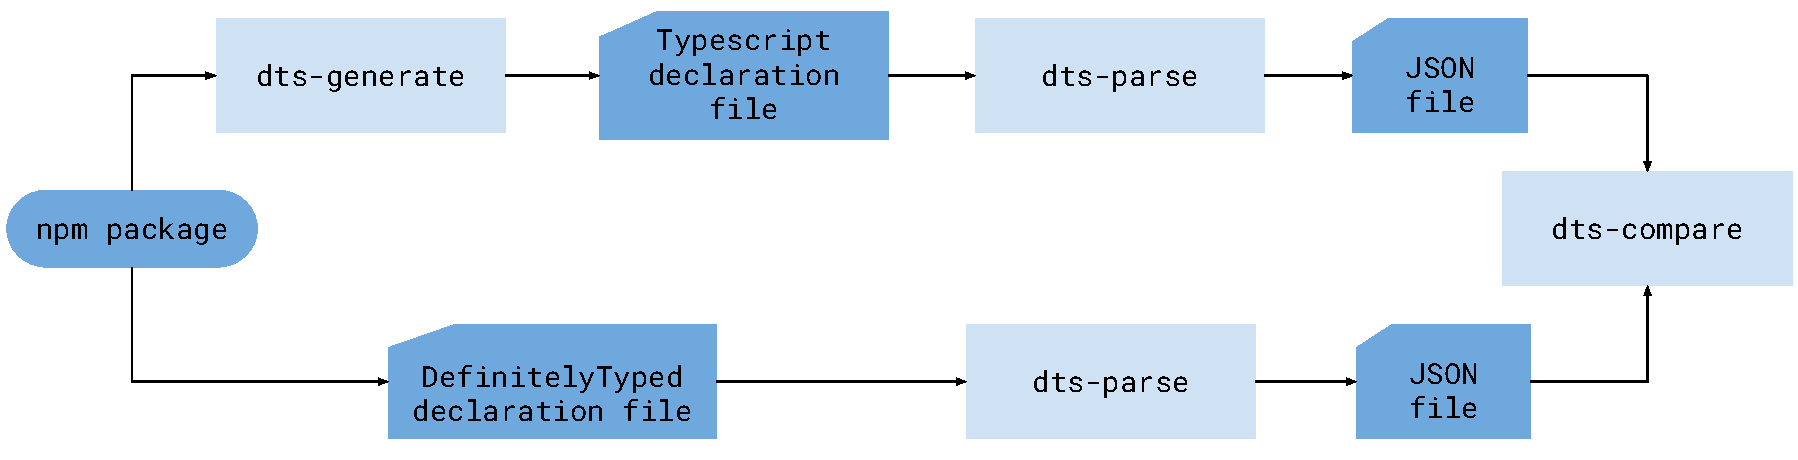
\includegraphics[width=1\linewidth]{evaluation-diagram.pdf}}
      \caption[Evaluation against DefinitelyTyped Repository]{\textbf{Evaluation of
          generated declaration files against DefinitelyTyped Repository} - The parser
        uses the TypeScript Compiler           API \cite{typescript-compiler-api} to
        transform declaration files into an abstract syntax which is serialized in
        JSON. The comparison is performed on the JSON format.} 
      \label{fig:evaluation-diagram}
  \end{centering}
\end{figure}

\subsection{dts-parse}
\label{sec:dts-parse}

We are not interested in a textual comparison of declaration files, but in a
comparison of the structures described by the
files. \texttt{dts-parse} receives the file as an input
parameter and returns an AST serialized in JSON.

The first step is to parse the declaration files using the TypeScript
Compiler API to build and traverse the 
Abstract Syntax Tree of a TypeScript program
\cite{typescript-compiler-api}. 
This step also performs a sanity check of the generated declaration
files as it rejects files with syntactic or semantic errors.
The output of \texttt{dts-parse} is a structure similar to a symbol table where declared
{interfaces}, {functions}, {classes}, and
{namespaces} are stored separately. Function arguments are
described, identifying complex types like union types or
callbacks. Optional parameters are also identified. For
{classes}, a distinction between constructors and methods
is made. Declaration files are tagged according to their features to identify and filter out declaration files
that contain unimplemented features.


% , as shown in \coderef{code:dts-parse-example}.
% \begin{lstlisting}[
%   caption={Example for \texttt{dts-parse} executed on module \texttt{glob-to-regexp} and combined with \texttt{jq} to browse the returned JSON},
%   language=bash,
% label=code:dts-parse-example,
%   float=tp, captionpos=b
% ]
% $ dts-parse -i glob-to-regexp/index.d.ts | jq '.parsing.functions[0].name'
% "GlobToRegexp"
% \end{lstlisting} %$

\subsection{dts-compare}
\label{sec:dts-compare}

% The tool is written in TypeScript.
The compare tool takes two declaration files as input and returns a
JSON file containing the result of the comparison as shown in
\coderef{code:dts-compare-example}. Following the naming convention of unit
testing frameworks, the input files are marked as \lstinline{expected} or
\lstinline{actual}. We use \lstinline{expected} for the DefinitelyTyped
declaration files. 

\begin{lstlisting}[
  caption={Example for \texttt{dts-compare} executed on declaration files without differences},
  language=bash,
label=code:dts-compare-example,
  float=tp,captionpos=b
]
$ dts-compare -e expected.d.ts -a actual.d.ts --module-name "my-module"
{
    "module": "my-module",
    "template": "module",
    "differences": [],
    "tags": []
}
\end{lstlisting}
% $

\texttt{dts-compare} applies \texttt{dts-parse} internally to both files to get 
normalized structures that are easy to compare. The result of the comparison is an array
of an abstract entity \texttt{Difference}. 
We classify a difference as \texttt{solvable} if it can be resolved by adding more code
examples. For example, we might add a function invocation with different parameters so that a missing
interface property gets accessed. Otherwise it is classified as  \texttt{unsolvable}. 

We consider the following differences:
\begin{itemize}
  \item \texttt{TemplateDifference}: A difference between the choice of TypeScript
    templates. For example, if the file in DefinitelyTyped is written as a \textbf{module}
    but we generated the file using the \textbf{module-function} template. The comparison
    stops if the templates differ. 
  \item \texttt{ExportAssignmentDifference}: An equality check between the export
    assignments of both files, that is in the expression
    \lstinline{export = XXX}.
  \item \texttt{FunctionMissingDifference}: A function declaration is present in the expected
    file but not in the generated one. This difference applies to functions as well as methods of classes
    and properties of interfaces. 
  \item \texttt{FunctionExtraDifference}: A function is present in the generated declaration file but not in DefinitelyTyped.
  \item \texttt{FunctionOverloadingDifference}: The number of declarations for the same
    function is different. This difference can be due to inexperience of the author of a
    declaration file, who uses, e.g., multiple declarations where a union typed argument
    would be appropriate.
  \item \texttt{ParameterMissingDifference}: A parameter of a function or a property of an interface is not present in the generated file.
  \item \texttt{ParameterExtraDifference}: A parameter of a function or a property of an
    interface is present in the generated file but not in the DefinitelyTyped file. 
  \item \texttt{ParameterTypeDifference}: A parameter of a function or a property of an interface is generated with a different type than in the DefinitelyTyped file. Here we differentiate between \texttt{SolvableDifference} and \texttt{UnsolvableDifference}.
  \begin{itemize}
    \item \texttt{SolvableDifference}: A type difference that can be solved by writing
      further code examples. For example, a basic type that is converted to a union type,
      a function overloading, or a parameter or property that is marked as optional. 
    \item \texttt{UnsolvableDifference}: Any difference not considered as \texttt{SolvableDifference}.
  \end{itemize}
\end{itemize}

Type aliases are expanded before the comparison and thus invisible to
\texttt{dts-compare}: the declaration
\lstinline{type T = string | number; declare function F(a: T);} is equivalent to
\lstinline{declare function} \lstinline{F(a: string | number);}. The same approach applies to literal
interfaces. \texttt{dts-compare} does 
not contemplate differences in function return types, because interface inference of
function return types is not covered in the current version of \texttt{dts-generate}. 

\section{Results}
\label{sec:results}
We analyzed the generated files focusing on the following aspects:
\begin{itemize}
  \item The quality of the inferred types, interfaces, and module structure using run-time information.
  \item The benefits of using code examples provided by developers as
    a first approximation to execute the libraries. %? and avoid a cold start problem.
  \item The usability of the generated declaration file and whether \texttt{dts-generate} can be used in a proper development environment.
\end{itemize}

\begin{quotation}
  The conducted experiments included tests that consisted of replacing
  a specific type definition from DefinitelyTyped
  \cite{definitely-typed-repository} with the one generated in the
  experiments: TypeScript compilation was successful, the generated
  JavaScript code ran without errors and code intelligence features
  performed by IDEs like code completion worked as expected.
\end{quotation}

Declaration files were generated for existing modules uploaded to the
\NPM{} registry. The DefinitelyTyped repository was used as a
benchmark. Each of the generated files was compared against the
corresponding declaration file uploaded to the repository.

Figure \ref{fig:experiments-overall-funnel} shows that a declaration file was generated
for \CountModulesGeneratedDeclarationFile{} modules out of
\CountTotalModulesDefinitelyTyped{} modules on DefinitelyTyped and we identified \CountModulesOnlySolvableDifferences{} modules that have only the
features implemented by \texttt{dts-generate}. We obtained positive results for all of
them. Section~\ref{sec:experiments-evaluation} provides a detailed explanation of the overall
quality of the generated files.
Section~\ref{sec:experiments-declaration-files-generation} presents examples of the generated declaration files for
templates \textbf{module}, \textbf{module-class}, and \textbf{module-function}.

\begin{figure}[tp]
  \centering
  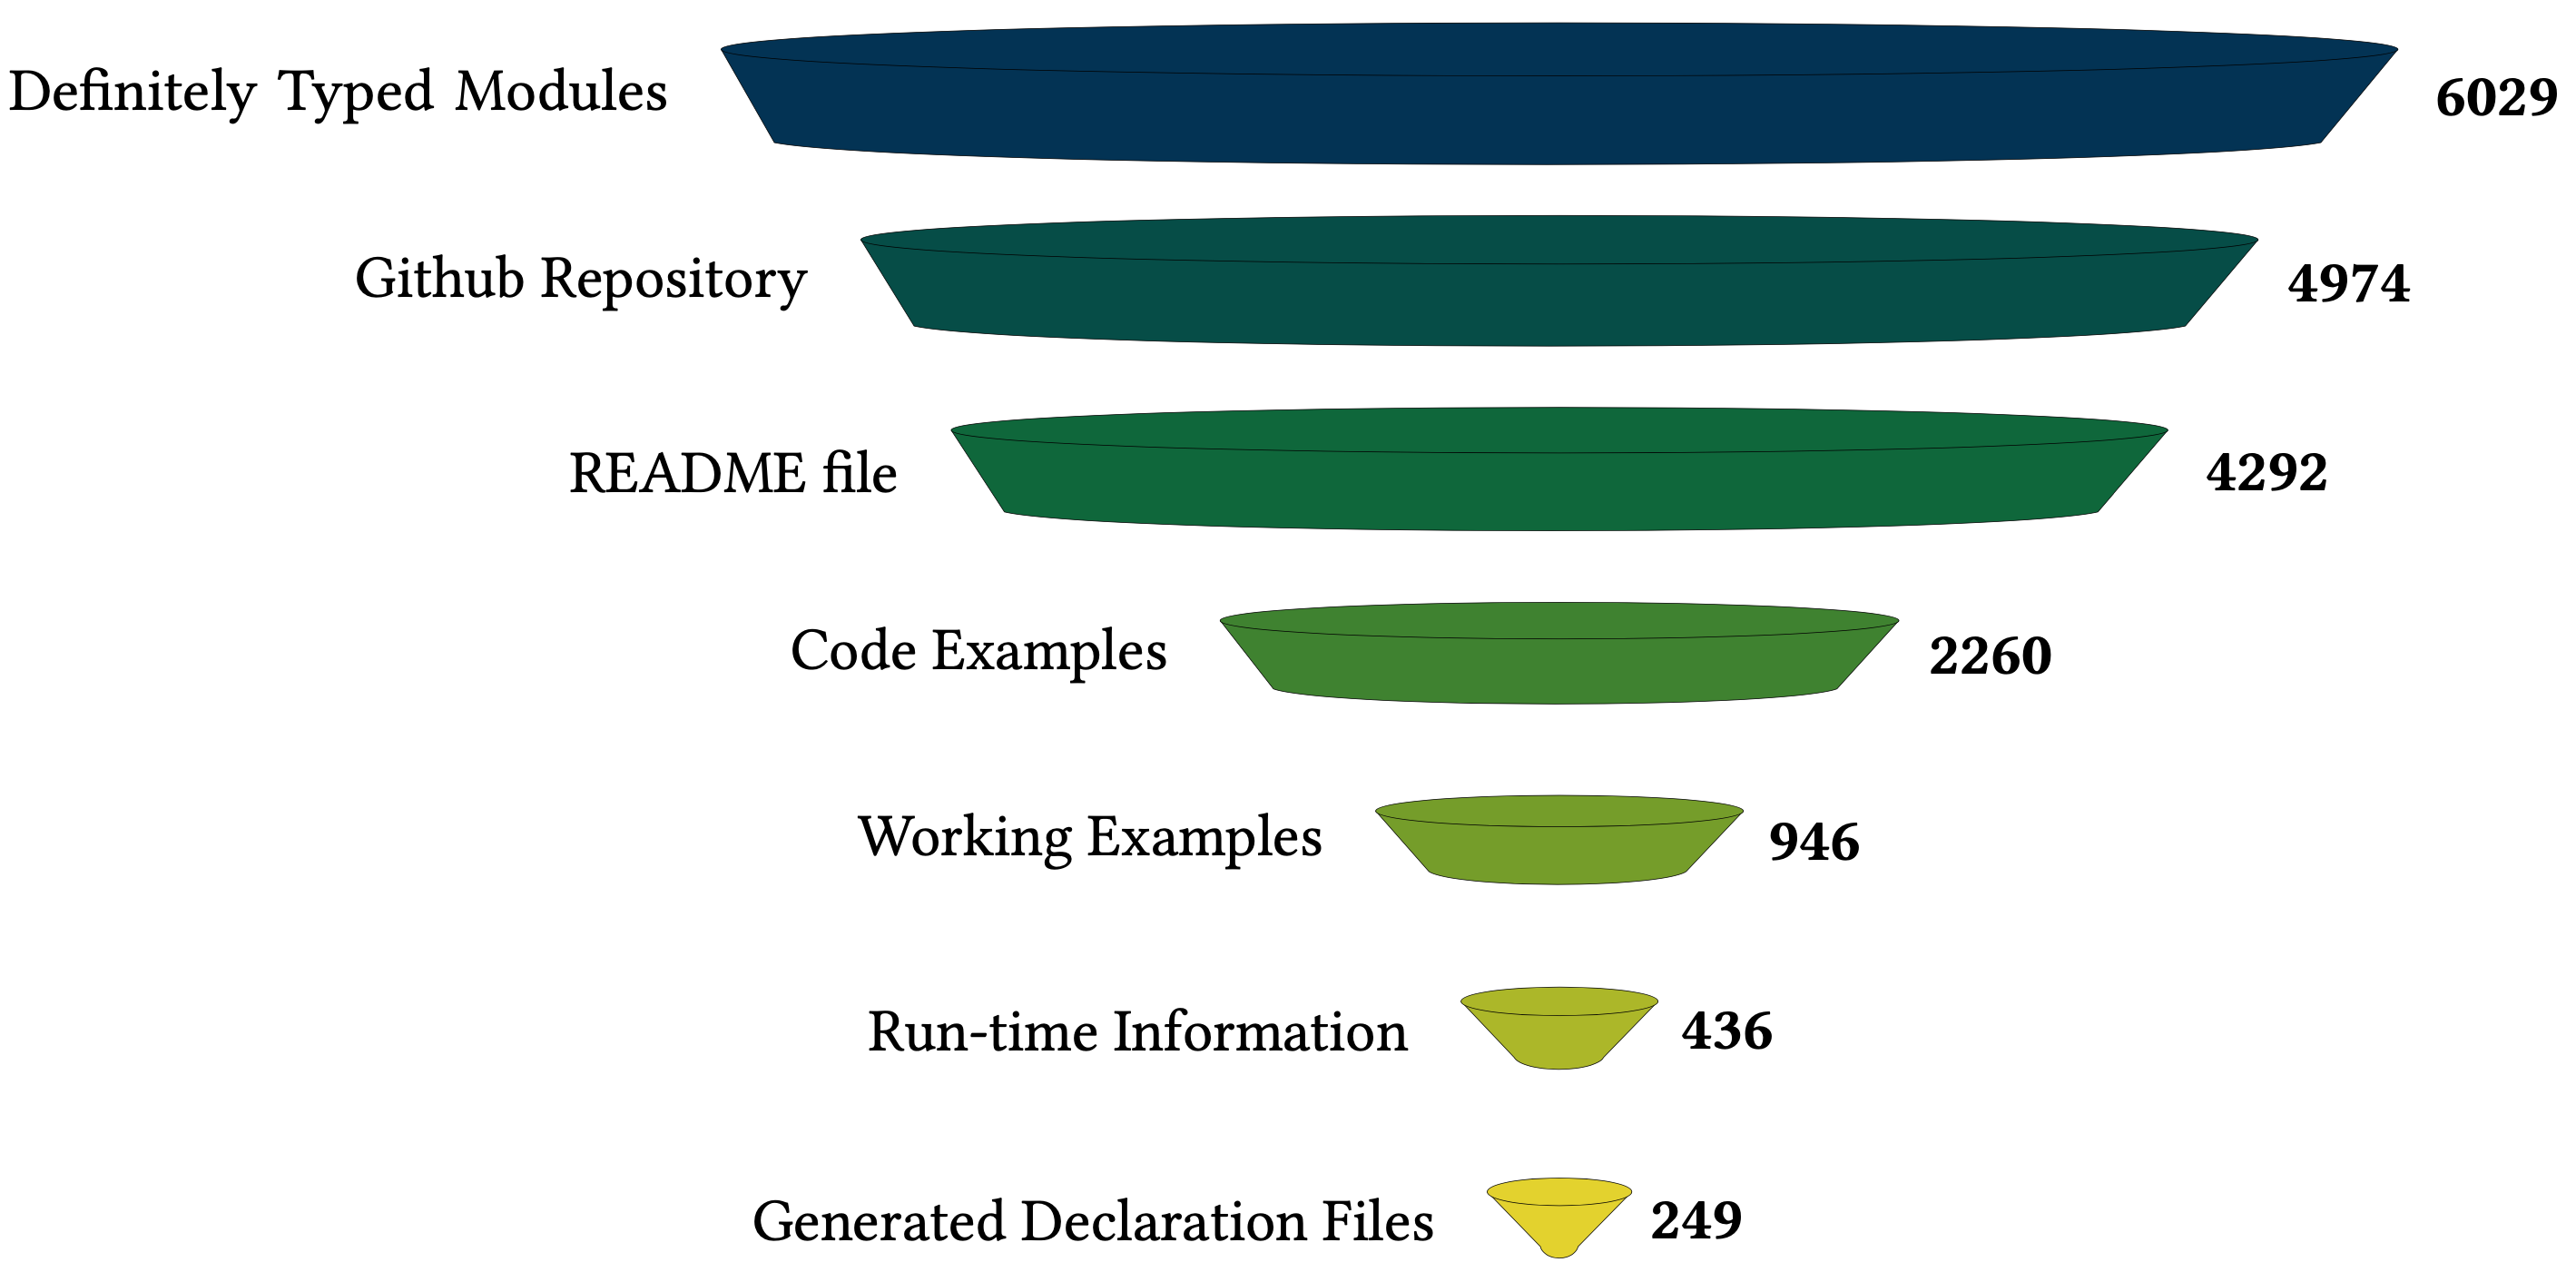
\includegraphics[width=1\linewidth]{funnel.png}
  \caption[Number of analyzed modules for each stage of the experiment]{
    \textbf{Number of analyzed modules for each stage of the experiment} - 
  A TypeScript Declaration File was generated for only \CountModulesGeneratedDeclarationFile{} modules, out of \CountTotalModulesDefinitelyTyped{} modules in the DefinitelyTyped Repository. 
  % It was only possible to gather valid run-time information for about 25\% of the modules for which a Code Example was extracted.
  } 
  \label{fig:experiments-overall-funnel}
\end{figure}

\subsection{Code Examples}
Retrieving the code examples for the JavaScript libraries proved to be
a pragmatic way of driving the type gathering at run time.
\figref{fig:experiments-overall-funnel} gives an overview of the
process to extract code examples. To understand why it was only possible
to obtain working code examples for \CountModulesWithCodeExamples{}
packages, we explain the steps in the process and analyze the losses
in each step.

The process of getting a valid code example for a module is divided in four
stages: 
\begin{itemize}
\item extracting the repository URL;
\item extracting a README file;
\item extracting code examples from README files;
\item executing code examples and discarding failing ones.
\end{itemize}

The results obtained for each step are described in the
following sections. 

\paragraph*{Repository URL}
The URL of the source repository could be retrieved for only \CountModulesWithRepositoryUrl{}
packages. More than 1000 packages on \NPM{} do not have a repository
entry in their corresponding \texttt{package.json} file. Therefore, the
\texttt{npm view <module> repository.url} command returns no
value. Even important modules like \texttt{ace} provide no repository URL.

\paragraph*{README Files}
\CountModulesWithoutReadmeFile{} packages do not have a README file in their repository, although
the implementation checks for several naming conventions like
\texttt{readme.md} or \texttt{README.md}. 

\paragraph*{Extraction of Code Examples}
In this step, we loose another 50\% of modules! This loss is mainly
explained because some developers do not wrap their code in a block
using the \texttt{javascript} or \texttt{js} tags. As we are
still left with code examples for \CountModulesWithCodeExamples{} modules, we did not look
further into code extraction as this number was considered sufficient for
evaluating the generation of declaration files. 

\paragraph*{Execution of Code Examples}
We executed the remaining \CountModulesWithCodeExamples{} extracted code examples by installing the
required packages and running the code as a \NodeJS{}
application. Unfortunately,
\CountModulesNotWorkingCodeExamples{} modules did not run correctly and had to be
discarded.
The code examples worked for the remaining \CountModulesWorkingCodeExamples{}
modules.
Some failing samples were analyzed and there were mainly
two reasons for the failure: 
\begin{itemize}
\item The code fragment had been properly extracted but the code was
  faulty. It invoked the library in an unsupported
  (obsolete?) way, which lead to a run-time error.
\item The extracted code fragment was not intended to be executed
  and/or it was not even valid JavaScript code. 
\end{itemize}

\paragraph*{Run-time Information}
Run-time information was extracted for only \CountModulesRunTimeInfoExtracted{} out of \CountModulesWorkingCodeExamples{} modules with working code
examples. As explained, to extract the run-time information, the behavior of the code
under analysis was explicitly modified by wrapping the arguments. Furthermore, Jalangi's
instrumentation itself caused some executions to fail, because the modules contained
JavaScript features that are not supported by Jalangi. As a result, run-time information
could not be extracted for \CountModulesRunTimeInfoCouldNotBeExtracted{} modules. An instrumentation without user-defined analysis
modules was not applied, so it was not possible to determine which modules were failing
only because of Jalangi's own limitations. 

\paragraph*{Generated Declaration Files}
A declaration file was generated for \CountModulesGeneratedDeclarationFile{} out of \CountModulesRunTimeInfoExtracted{} modules. Despite the correct execution
of the instrumented code examples, \CountModulesDeclarationFileCouldNotBeGenerated{} modules did not yield suitable run-time information
for generating a declaration file. The extracted code examples for these modules did not
execute the library. Hence, the collected run-time information was not sufficient
for generating a declaration file. 

\subsection{Declaration Files Generation}
\label{sec:experiments-declaration-files-generation}

This section exhibits some examples of the \CountModulesGeneratedDeclarationFile{} generated
declaration files. It shows some results for each of the implemented
templates: \textbf{module}, \textbf{module-function}, and
\textbf{module-class}. 

\figref{fig:experiments-results-module-function} shows the generated
declaration files for simple modules like \texttt{abs},
\texttt{dirname-regex}, and \texttt{escape-html}. All of them were
generated using the \textbf{module-function} template. The left side of the figure shows
the generated declaration file with 
\lstinline{dts-generate}, the right side shows the corresponding file
in the DefinitelyTyped repository. 
There are no relevant differences between the files. 
The different names in the export assignment by modules \texttt{dirname-regex} and
\texttt{escape-html} do not matter because the module can be named arbitrarily when it is imported: in
\lstinline[language=TypeScript]/import Abs = require('abs');/ the
identifier \lstinline[language=TypeScript]/Abs/ can be chosen by the
programmer. We generate the name in the export 
assignment by transforming the module name into camel case form, following TypeScript
guidelines.

Functions are correctly detected; input and output types are
accurately inferred. 
We extract the parameter names from the variable names of the JavaScript
code.
A difference in the names of the function parameters does not affect the correctness of
the declaration file.
Furthermore, neither the order of declarations nor unused namespaces
(as in module \texttt{escape-html}) matter.

 
\begin{figure*}[tp]
    \centering
    \begin{subfigure}[t]{0.48\linewidth}
      \begin{lstlisting}[language=TypeScript,numbers=none]
export = Abs;

declare function Abs(input: string): string;
      \end{lstlisting}
      \caption{abs/index.d.ts - Generated}
    \end{subfigure}
    \hfill
    \begin{subfigure}[t]{0.48\linewidth}
      \begin{lstlisting}[language=TypeScript,numbers=none]
declare function Abs(input: string): string;
export = Abs;
      \end{lstlisting}
      \caption{abs/index.d.ts - DT}
    \end{subfigure}


    \begin{subfigure}[t]{0.48\linewidth}
        \begin{lstlisting}[language=TypeScript,numbers=none]
export = DirnameRegex;

declare function DirnameRegex(): RegExp;
        \end{lstlisting}
        \caption{dirname-regex/index.d.ts - Generated}
      \end{subfigure}
      \hfill
      \begin{subfigure}[t]{0.48\linewidth}
        \begin{lstlisting}[language=TypeScript,numbers=none]
export = dirnameRegex;

declare function dirnameRegex(): RegExp;
        \end{lstlisting}
        \caption{dirname-regex/index.d.ts - DT}
      \end{subfigure}


      \begin{subfigure}[t]{0.48\linewidth}
        \begin{lstlisting}[language=TypeScript,numbers=none]
export = EscapeHtml;

declare function EscapeHtml(string: string): string;

        \end{lstlisting}
        \caption{escape-html/index.d.ts - Generated}
      \end{subfigure}
      \hfill
      \begin{subfigure}[t]{0.48\linewidth}
        \begin{lstlisting}[language=TypeScript,numbers=none]
declare function escapeHTML(text: string): string;
declare namespace escapeHTML { }

export = escapeHTML;
        \end{lstlisting}
        \caption{escape-html/index.d.ts - DT}
      \end{subfigure}

    \caption{Results for \textbf{module-function} template}
    \label{fig:experiments-results-module-function}
\end{figure*}


\begin{figure*}[tp]
  \centering
  \begin{subfigure}[t]{0.48\linewidth}
    \begin{lstlisting}[language=TypeScript,numbers=none]
export function v1(str: string): boolean;
export function v2(str: string): boolean;
export function v3(str: string): boolean;
export function v4(str: string): boolean;
export function v5(str: string): boolean;
    \end{lstlisting}
    \caption{is-uuid/index.d.ts - Generated}
  \end{subfigure}
  \hfill
  \begin{subfigure}[t]{0.48\linewidth}
    \begin{lstlisting}[language=TypeScript,numbers=none]
export function v1(value: string): boolean;
export function v2(value: string): boolean;
export function v3(value: string): boolean;
export function v4(value: string): boolean;
export function v5(value: string): boolean;
export function nil(value: string): boolean;
export function anyNonNil(value: string): boolean;
    \end{lstlisting}
    \caption{is-uuid/index.d.ts - DT}
  \end{subfigure}

  \caption{Results for \textbf{module} \texttt{is-uuid}}
  \label{fig:experiments-results-module-is-uuid}
\end{figure*}

\figref{fig:experiments-results-module-is-uuid} contains an example
for the \textbf{module} template, the declaration for the \texttt{is-uuid} module.
The generated file only contain methods that were executed by the extracted
examples. All invoked functions are correctly detected; the additional
functions declared on DefinitelyTyped are not used in the example
code.
It would be easy to generate a perfectly matching declaration file by
adding two examples using functions \texttt{nil} and
\texttt{anyNonNil}. 

% This is no longer true. I'll add one result to the report.
We were unable to  generate a declaration file based on the
\textbf{module-class} template. All modules corresponding to this template exhibited at least one of
the unimplemented TypeScript features. 

It is worth mentioning that for some libraries the declaration file in DefinitelyTyped was
not correct. For example, for the module \texttt{glob-base}, the parameter
\texttt{basePath} is declared as optional in DefinitelyTyped. However, when invoking the
function without the \texttt{basePath} parameter, an error is thrown at run time. The file generated by
\texttt{dts-generate} does not mark this parameter as optional, as shown in
\figref{fig:experiments-results-module-glob-base}. Function return type interfaces are
not inferred by \texttt{dts-generate}.
% The parameter name is \texttt{pattern}
% instead of \texttt{basePath}, because the JavaScript implementation declares the parameter
% as \texttt{pattern}, as shown in \figref{fig:subfloat-globbase-js-implementation}. 
We also
discovered errors in the selected template in DefinitelyTyped. The module
\texttt{smart-truncate} in DefinitelyTyped uses the \textbf{module} template, but
\texttt{dts-generate} generates a file using the \textbf{module-function}
template. \coderef{code:experiments-results-module-smart-truncate} shows that the module is indeed
exported as a function, as inferred by \texttt{dts-generate}.

\begin{figure*}[tp]
  \centering
  \begin{subfigure}[t]{0.48\linewidth}
    \begin{lstlisting}[language=TypeScript,numbers=none]
'use strict';

// ...

module.exports = function globBase(pattern) {
if (typeof pattern !== 'string') {
  throw new TypeError('glob-base expects a string.');
}

// ...
} 
    \end{lstlisting}
    \caption{glob-base/index.js - Excerpt of JS implementation
      that throws an Error when input parameter is not a string} 
    \label{fig:subfloat-globbase-js-implementation}
  \end{subfigure}
  \hfill
  \begin{subfigure}[t]{0.48\linewidth}
    \begin{lstlisting}[language=TypeScript,numbers=none]
declare function globbase(basePath?: string): globbase.GlobBaseResult;

declare namespace globbase {
  interface GlobBaseResult {
      base: string;
      isGlob: boolean;
      glob: string;
  }
}

export = globbase;
    \end{lstlisting}
    \caption{glob-base/index.d.ts - DefinitelyTyped}
  \end{subfigure}

\begin{subfigure}[t]{0.48\linewidth}
    \begin{lstlisting}[language=JavaScript,numbers=none]
var globBase = require('glob-base');

globBase();

// Throws: TypeError: glob-base expects a string.
    \end{lstlisting}
    \caption{Code example invoking the exported function without the first parameter, as specified in DefinitelyTyped}
  \end{subfigure}
  \hfill
  \begin{subfigure}[t]{0.48\linewidth}
    \begin{lstlisting}[language=TypeScript,numbers=none]
export = GlobBase;

declare function GlobBase(pattern: string): object;
    \end{lstlisting}
    \caption{glob-base/index.d.ts - Generated}
  \end{subfigure}
  
  \caption{Incorrect optional parameter for module \texttt{glob-base}}
  \label{fig:experiments-results-module-glob-base}
\end{figure*}

\begin{lstlisting}[
caption={Code example for \texttt{smart-truncate} module exporting a function},
label=code:experiments-results-module-smart-truncate,
language=JavaScript,captionpos=b,float=tp,numbers=none
]
var smartTruncate = require('smart-truncate');

var string = 'To iterate is human, to recurse divine.';

// Append an ellipsis at the end of the truncated string.
var truncated = smartTruncate(string, 15);
\end{lstlisting}

\subsection{Evaluation}
\label{sec:experiments-evaluation}
We analyzed \CountModulesOnlySolvableDifferences{} of the \CountModulesGeneratedDeclarationFile{} generated files. The remaining 174 files contained at least one
of the unimplemented TypeScript features so that they could not be
considered.
% ? These features were identified by \texttt{dts-parse} as tags.


As shown in \figref{fig:experiments-results-module-is-uuid}, the code examples have a
direct influence on the quality of the generated declaration file. We introduced the
concept of \texttt{solvable} and \texttt{unsolvable} differences in
\secref{sec:dts-compare}. Modules containing only \texttt{solvable} differences were
considered as positive results. All of the analyzed files contained only \texttt{solvable} differences. We manually completed the
examples for 10 of those modules. Applying \texttt{dts-generate} with the completed
examples generates declaration files, which are equivalent to the files from DefinitelyTyped, as
shown in \figref{fig:experiments-results-manually-completed-examples}.

\begin{figure*}[t]
  \centering
  \begin{subfigure}[t]{0.45\linewidth}
    \begin{lstlisting}[language=TypeScript]
declare namespace gh {
  interface Options {
      enterprise?: boolean;
  }
  interface Result {
      ...
  }
}

declare function gh(url: string | {url: string}, options?: gh.Options): gh.Result | null;

export = gh;    
    \end{lstlisting}
    \caption{github-url-to-object/index.d.ts - DefinitelyTyped. Properties of interface \texttt{Result} were ignored for readability, since return types were not considered.}
  \end{subfigure}
  \hfill
  \begin{subfigure}[t]{0.45\linewidth}
    \begin{lstlisting}[language=TypeScript]
export = GithubUrlToObject;

declare function GithubUrlToObject(repoUrl: string | GithubUrlToObject.I__repoUrl, opts?: GithubUrlToObject.I__opts): object | null;
declare namespace GithubUrlToObject {
  export interface I__repoUrl {
    'url'?: string;
  }

  export interface I__opts {
    'enterprise'?: boolean;
  }

}
    \end{lstlisting}
    \caption{github-url-to-object/index.d.ts - Generated with manually expanded code example}
  \end{subfigure}

  \begin{subfigure}{0.80\linewidth}
    \begin{lstlisting}[language=JavaScript]
var gh = require('github-url-to-object')

gh('github:monkey/business');
gh('https://github.com/monkey/business');
gh('https://github.com/monkey/business/tree/master');
gh('https://github.com/monkey/business/tree/master/nested/file.js');
gh('https://github.com/monkey/business.git');
gh('http://github.com/monkey/business');
gh('git://github.com/monkey/business.git');

// Manually added:
gh('git+https://githuuub.com/monkey/business.git', {});
gh('git+https://githuuub.com/monkey/business.git', {enterprise: true});
gh({url: 'git://github.com/monkey/business.git'});
gh('this is not a proper url');
gh({url: 'this is not a proper url'});
    \end{lstlisting}
    \caption{Code example for module \texttt{github-url-to-object}.}
    \end{subfigure}
  \caption{Manually expanded code example for
    \texttt{github-url-to-object} to match DefinitelyTyped declaration
    file. The literal interface in DefinitelyTyped is replaced by a
    declared interface. Return types are not considered.} 
  \label{fig:experiments-results-manually-completed-examples}
\end{figure*}

\section{Discussion}
\label{sec:discussion}

How can we improve further? Given that JavaScript developers are incentivized to develop good
examples rather than writing ``boring'' type declarations, how can we capitalize on that attitude?
The main issue is that any example-driven algorithm can only come up with an
under-approximation of the intended meaning, so some form of help is required when
generalization is desired.

\paragraph*{Literal types vs string}
Many JavaScript libraries use literal strings to select
options and configurations. To be concrete, 1925 DT packages rely on
literal types (see Table~\ref{tab:dts-parse-stats}). For example, the bonjour
package\footnote{\url{https://www.npmjs.com/package/@types/bonjour}}
relies on strings to control events and indicate protocols in (different) interfaces:
\begin{lstlisting}[language=TypeScript]
    removeAllListeners(event?: 'up' | 'down'): this;
    protocol?: 'udp'|'tcp';
\end{lstlisting}
The carlo
package\footnote{\url{https://www.npmjs.com/package/@types/carlo}}
uses it to distinguish different 
types of events.
\begin{lstlisting}[language=TypeScript]
export type AppEvent = 'exit' | 'window';
\end{lstlisting}
% coinbase ...

For our framework, it is hard to distinguish a string that is meant literally from a
string that just serves as an example. For an automatic solution, one might collect
typical values of literal strings and generate the corresponding literal types (or
unions thereof) when the arguments used in the example are all typical. Alternatively, one
might always generate literal types unless the number of different examples provided is
greater than some threshold, in which case the generator generalizes to type
\lstinline/string/. Both alternatives come with the problem that they
create a local over-approximation, so that it would become harder to
qualify the output of the generator. A further alternative that does
not suffer from this drawback would be to communicate to the developer a set
of typical example strings, \emph{marker strings}, that the generator
always generalizes to the \lstinline/string/ type.

\paragraph*{Any}
Suppose the programmer supplies examples that use \lstinline/number/, \lstinline/bool/, and
\lstinline/string/ at the same argument position. The obvious approximation to the type of
this argument is the union type \lstinline/number|bool|string/. But what if the programmer
wants to advertise the type \lstinline/any/ for an argument? This intent is hard to
communicate with a finite number of examples.

We propose that the programmer relies on marker strings like \lstinline/"any"/ to indicate
the \lstinline/any/ type for an argument position.

\paragraph*{Further types}
Similar approaches could be conceived for indexed types, polymorphic types, dependent
types, etc. However, at present we believe incorporating these features in a tool to be
overblown because they are not widely used in DefinitelyTyped (see
Table~\ref{tab:dts-parse-stats}). 

\section{Related Work}
\label{sec:related-work}
\paragraph*{dts-gen}
TypeScript comes with \texttt{dts-gen}, a tool that creates declaration files for
JavaScript libraries \cite{dts-gen}. Its documentation states that the result is 
intended to be used as a starting point for the development of a declaration file. The outcome
needs to be refined afterwards by the developer. 

The tool analyzes the shape of the objects at runtime after initialization without
executing the library. This results in most parameters and results being inferred as
\lstinline[language={}]{any}.
% \coderef{code:related-work-dts-gen-example} shows an example
% for module \lstinline[language={}]{abs}. 

In contrast, our tool \texttt{dts-generate} is intended to generate declaration files
that are ready to be uploaded to DefinitelyTyped without further manual intervention. Any
amount of manual work that a developer needs to do on a declaration file after updating
JavaScript code increases the risk of discrepancies between the declaration file
and the implementation.

% Formal aspects like applying the right template and using the correct syntax are perfectly covered by \texttt{dts-gen}.

%$ npm i -g dts-gen
% $ npm i -g abs
% $ dts-gen -m abs
% Wrote 5 lines to abs.d.ts.

% $ cat abs.d.ts

% \begin{lstlisting}[
%     language=TypeScript,
%     caption={Microsoft's dts-gen example - A declaration file for
% module \lstinline!abs! is generated. Types are inferred as
% \lstinline!any!. The correct \textbf{module-function} template is
% used.}, 
% 	label=code:related-work-dts-gen-example,
%     float=tp,captionpos=b
% ]
% /** Declaration file generated by dts-gen */

% export = abs;

% declare function abs(input: any): any;
% \end{lstlisting}

\paragraph*{TSInfer \& TSEvolve}
TSInfer and TSEvolve are presented as part of TSTools
\cite{DBLP:conf/fase/KristensenM17}. Both tools are the continuation of TSCheck
\cite{DBLP:conf/oopsla/FeldthausM14}, a tool for detecting mismatches between a
declaration file and the implementation of the module. 

TSInfer proceeds in a similar way than TSCheck. It initializes the library in a browser
and records a snapshot of the resulting state.  Then it performs a lightweight static
analysis on all the functions and objects stored in the snapshot. 

The abstraction and the constraints introduced as part of the static analysis tools
for inferring the types have room for improvement. A run-time based approach like the one
presented in our work will provide more accurate information, thus generating more precise
declaration files.

As TSInfer analyzes the objects and functions stored in the snapshot, it faces the problem
of including internal methods and private properties in the declaration file. Run-time
information would have informed that the developer has no intention of exposing these
methods. 

Moreover, TSEvolve performs a differential analysis on the changes made to a JavaScript
library to determine intentional discrepancies between the declaration files of two
consecutive versions. However, a differential analysis may not be needed. If the
developer's intention were accurately represented by the extracted code, then the generated
declaration file would already describe the newer version of a library without the need of
a differential analysis.

\paragraph*{TSTest}
TSTest is a tool that checks for mismatches between a declaration file and the JavaScript
implementation of the module \cite{DBLP:journals/pacmpl/KristensenM17}. It applies feedback-directed
random testing for generating type test scripts. These scripts execute the library with
random arguments with the typings from the declarations file and check whether the output
matches the prescribed type. TSTest thus provides concrete counterexamples if it detects mismatches.

% We evaluated the generated declaration files comparing them to the declaration files
% uploaded to DefinitelyTyped. The disadvantage of doing this is that since the uploaded
% files are written manually, they could already contain mismatches with the JavaScript
% implementation. However, it is a suitable choice for a development stage since it is used
% as a baseline.

% In a final stage, declaration files need to be checked against the proper JavaScript
% implementation and TSTest has to be definitely taken into account. 

TSTest could be used to extend our tool with a feedback loop. If TSTest detects a problem
with a declaration file generated by \texttt{dts-generate}, then we would add the
resulting counterexamples to the example code and restart the generation process. 

\section{Conclusions and Future Work}
\label{sec:conclusion}
We have presented \texttt{dts-generate}, a tool for generating a TypeScript declaration
file for a specific JavaScript library. The tool downloads code examples written by the
developers from the library's repository. It uses these examples to execute the library and
gather data flow and type information. The tool finally generates a TypeScript declaration
file based on the information gathered at run time.

We developed an architecture that supports the automatic generation of declaration files
for specific JavaScript libraries without additional manual tasks. The architecture
contemplates future incorporation of a Symbolic Execution Engine that refines the
initial code base enabling the exploration of new execution paths. Although it is not
implemented 
in this work, its incorporation would result in small incremental modifications to the
presented architecture as it is considered to only expand the existing code base.

Building an end-to-end solution for the generation of TypeScript declaration files was
prioritized over type inference accuracy. Consequently, types were taken over from the
values at run time. Developers express their intent how a library should be used with
example code in the documentation. Hence,
obtaining the types from the code examples extracted from the repositories proved to be a
pragmatic and effective approximation, enabling to work on specific aspects regarding the
TypeScript declaration file generation itself.

We built a mechanism to automatically create declaration files for potentially every
module uploaded to DefinitelyTyped. We managed to generate declaration files for
\CountModulesGeneratedDeclarationFile{} modules. We compared the results against the corresponding 
files uploaded to
DefinitelyTyped by creating \texttt{dts-parse}, a TypeScript declaration files parser and
\texttt{dts-compare}, a comparator.

% \begin{changethis}
%   We exposed the fundamental aspect of capturing the developer's intention when inferring
%   types in JavaScript. Instead of applying constraints and restrictions for operations
%   with certain types, we presented a proposal that favors best practice. Uncommon usage is
%   not forbidden but greatly discouraged. Accordingly, we collected evidence regarding the
%   usage of JavaScript operators by analyzing 400 libraries.
% \end{changethis}

% Finally, the architecture is composed of different blocks that interact with each
% other. Each block is independent and has a well defined behavior as well as clear input
% and output values. As a result, each block can be independently and simultaneously
% improved.

%%
%% The next two lines define the bibliography style to be used, and
%% the bibliography file.
\bibliographystyle{ACM-Reference-Format}
\bibliography{main}

\end{document}
\endinput
%%
%% End of file `sample-sigconf.tex'.
